\paragraph{Reflective system.}

%De nombreux langages r\'eflexifs sont apparus ces derni�res ann\'ees : langages
%objets \cite{Maes87a, Bobr86a, Coint87a, Coint89a, Chiba93a, Danforth94a,
%Chiba95, Brandt96, Rivard96b}, langages d'acteurs \cite{Ferber84,Ferber88,
%Ferber93, Briot94, Briot96}, programmation concurrente \cite{Yonezawa88,
%Ishikawa91,Yonezawa92, Yonezawa92b}, langages � prototypes \cite{Mulet93a,
%Mulet93b, Mulet95}.  L'utilisa\-tion de protocoles m\'eta-objet a permis de mettre
%en place des m\'ecanismes vari\'es comme des types de donn\'ees atomiques
%\cite{Stroud95}, l'introduction d'objets persistants \cite{Paepcke90}, des
%bo�tes � outils graphiques \cite{Rao91,Gallesio96} et la construction de
%syst�mes d'exploitation.  Apr�s avoir pos\'e le vocabulaire, nous analysons les
%besoins qui ont favoris\'e l'\'emergence des syst�mes dit {\em ouverts}.  Nous
%abordons ensuite les difficult\'es sp\'ecifiques � la conception de ces syst�mes.
%Nous pr\'esentons rapidement deux protocoles m\'eta-objet (MOP) en pr\'esentant
%celui de \Clos \cite{Kiczales91} et de \CodA \cite{McJaffer95}.  Nous avons
%choisi \Clos car son MOP constitue la r\'ef\'erence en la mati�re, mais aussi le
%MOP nomm\'e \CodA qui choisit une factorisation des m\'eta-comportements originale
%et plus g\'en\'erale centr\'ee autour du concept d'objet. 
%

%\section{Concepts et d\'efinitions}
%\mcite{La r\'eflexion d\'esigne l'ensemble des pr\'eoccupations visant � rendre
%visible dans le langage certains m\'ecanismes internes.}{Mulet95}
%
%La r\'eflexion est � la base des langages ouverts.  Ce concept qui ne se limite
%pas exclusivement aux langages � objets existe aussi en programmation logique
%ou fonctionnelle \cite{Demers95}.  \Smith fut le premier � introduire un tel
%concept dans un langage de programmation : \tLisp, son langage r\'eflexif, \'etait
%un langage fonctionnel \Lisp \cite{Smith84}. 


Smith defines reflexivity as: {\em <<~An entity's integral ability to represent, operate on, and
otherwise deal with itself in the same way that it represents, operates on and
deals with its primary subject matter~>>}.~\cite{Bobr93a}

In the context of programming languages, this definition can be stated
as: \emph{Reflection is the ability of a program to manipulate as data
something representing the state of the program during its own
execution. There are two aspects of such manipulation : {\em introspection}
and {\em intercession} [...] Both aspects require a mechanism for encoding
execution state as data; providing such an encoding is called {\em
reification}.}~\cite{Bobr93a}


Maes has proposed in the first chapter of his thesis
\cite{Maes87b}, precise definitions to clearly characterize
reflective programming. We refer here to these definitions:

\begin{itemize}
\item A {\bf computational system} is something that {\bf reasons} about and
{\bf acts} upon some part of the world, called the {\bf domain} of the system
(p 13).

\item A computational system may also be {\bf causally connected} to its
domain. This means that the system and its domain are linked in such a way
that if one of the two changes, this leads to an effect upon the other (p 15).

\item A {\bf meta-system} is a computational system that has as its domain
another computational system, called its {\bf object-system}. [...] A
meta-system has a representation of its object-system in its data. Its
program specifies {\bf meta-computation} about the object-system and is
therefore called a {\bf meta-program} (p 17).

\item {\bf Reflection} is the process of reasoning about and/or acting upon
oneself (p 19) (see Figure~\ref{AllSystems}).

\begin{figure}[h]
	\centering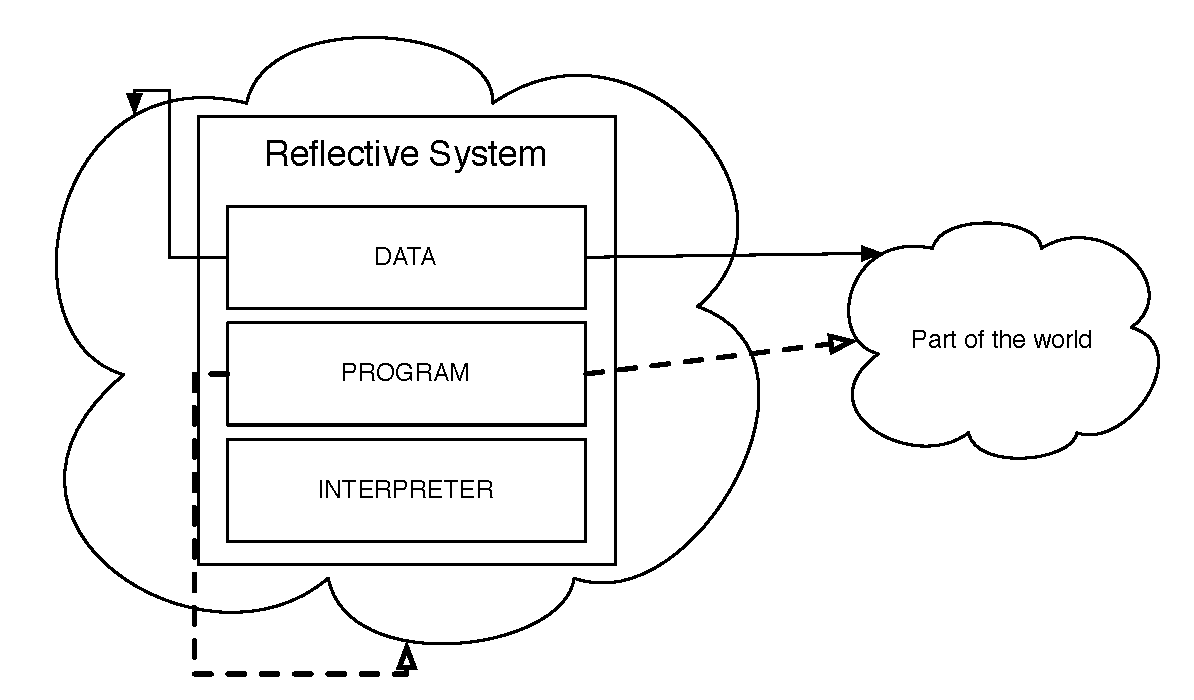
\includegraphics[width = 10cm]{figures/ReflexiveSystem}
	\caption{A Reflexive System}
	\label{AllSystems}
\end{figure}



\item A {\bf reflective system} is a causally connected meta-system that has
as object-system itself. The data of a reflective system contain, besides the
representation of some part of the external world, also a causally connected
representation of itself, called {\bf self-representation} of the
system. [...] When a system is reasoning or acting upon itself, we speak of
{\bf reflective computation} (p 19).

\item A language with a {\bf reflective architecture} is a language in which
all systems have access to a causally connected representation of themselves.

\item A programming environment has a {\bf meta-level architecture} if it has
an architecture which supports meta-computation, without supporting reflective
computation (p 34).
\item The {\bf meta-object} of an object X represents the explicit information
about X (e.g. about its behavior and its implementation). The object X itself
groups the information about the entity of domain it represents (p 120).
\end{itemize}

\paragraph{Bootstrap.}
Bootstrapping a kernel is the process that builds the minimal structure of a language that is reusable to define this language.
The idea is to use as early as possible the benefits of the resulting language by implementing a minimal core whose only goal is to be able to build the full system. As an example of a possible bootstrap: we write in C the minimal structures to represent and execute objects, and we then write with this core the full system. This avoids to have to write the full system (compiler for example in C). In ObjvLisp \cite{Coin87a}, the class Class is first defined using low level API, then Object is created, then Class is fully reimplemented using the first one.